\documentclass[a4paper]{article}
\usepackage[utf8]{inputenc}
\usepackage[dvipsnames]{xcolor}
\usepackage[hidelinks]{hyperref}
\usepackage{graphicx, amssymb, amsfonts, color, todonotes, diagbox, colortbl, pdfpages, listings, amsmath, caption, subcaption, xspace, xcolor, pifont, fullpage, algorithm, algpseudocode}
\algnewcommand\algorithmicforeach{\textbf{for each}}
\algdef{S}[FOR]{ForEach}[1]{\algorithmicforeach\ #1\ \algorithmicdo}
\setlength{\parskip}{0.2 cm}
\newtheorem{definition}{Definition}
\newtheorem{theorem}{Theorem}
%~ \usepackage{amsmath}
% Commands
\newcommand{\Node}[1]{\ensuremath{\mathrm{Node}_{#1}}\xspace}
\newcommand{\flow}[1]{\ensuremath{\mathit{flow}_{#1}}\xspace}
\newcommand{\inputs}{\ensuremath{\mathcal{F}}\xspace}
\newcommand{\memory}{\ensuremath{\mathcal{M}}\xspace}
\newcommand{\memorymap}{\ensuremath{\mathcal{M}_{map}}\xspace}
\newcommand{\duration}{\mathit{Duration}\xspace}
\newcommand{\bandwidth}{\mathit{BW}\xspace}
\newcommand{\core}{\mathit{Cores}\xspace}
\newcommand{\submissiontime}{\mathit{Subtime}\xspace}
\newcommand{\walltime}{\mathit{Walltime}\xspace}
\newcommand{\completiontime}{\mathit{Completiontime}\xspace}
\newcommand{\start}{\mathit{Starttime}\xspace}
\newcommand{\fileset}{\ensuremath{\mathbb{F}}\xspace}
\newcommand{\jobset}{\ensuremath{\mathbb{J}}\xspace}
\newcommand{\nodeset}{\ensuremath{\mathbb{N}}\xspace}
\newcommand{\evict}{\ensuremath{\mathcal{V}}\xspace}
\newcommand{\nbloads}{\ensuremath{\mathit{\mathit{Loads}}}\xspace}
\newcommand{\live}{\ensuremath{L}\xspace}
\renewcommand{\algorithmicrequire}{\textbf{Input:}}
\renewcommand{\algorithmicensure}{\textbf{Output:}}

\begin{document}

\begin{figure}[H]\centering
\begin{subfigure}[b]{0.4\linewidth}\centering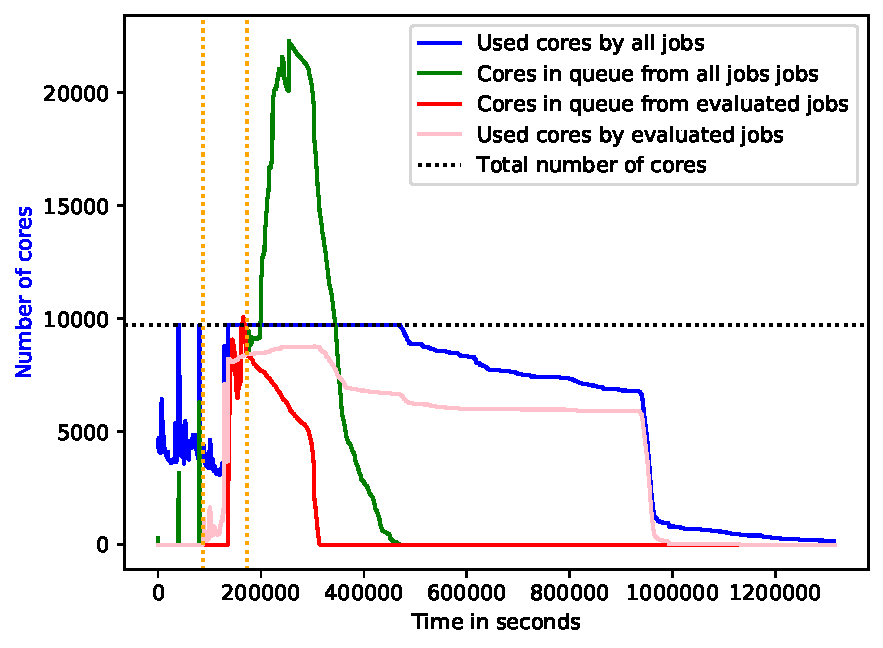
\includegraphics[width=1\linewidth]{MBSS/plot/2022-07-18->2022-07-18_V9271_Fcfs_Used_nodes_450_128_32_256_4_1024.pdf}\caption{Cluster's usage}\end{subfigure}
\begin{subfigure}[b]{0.4\linewidth}\centering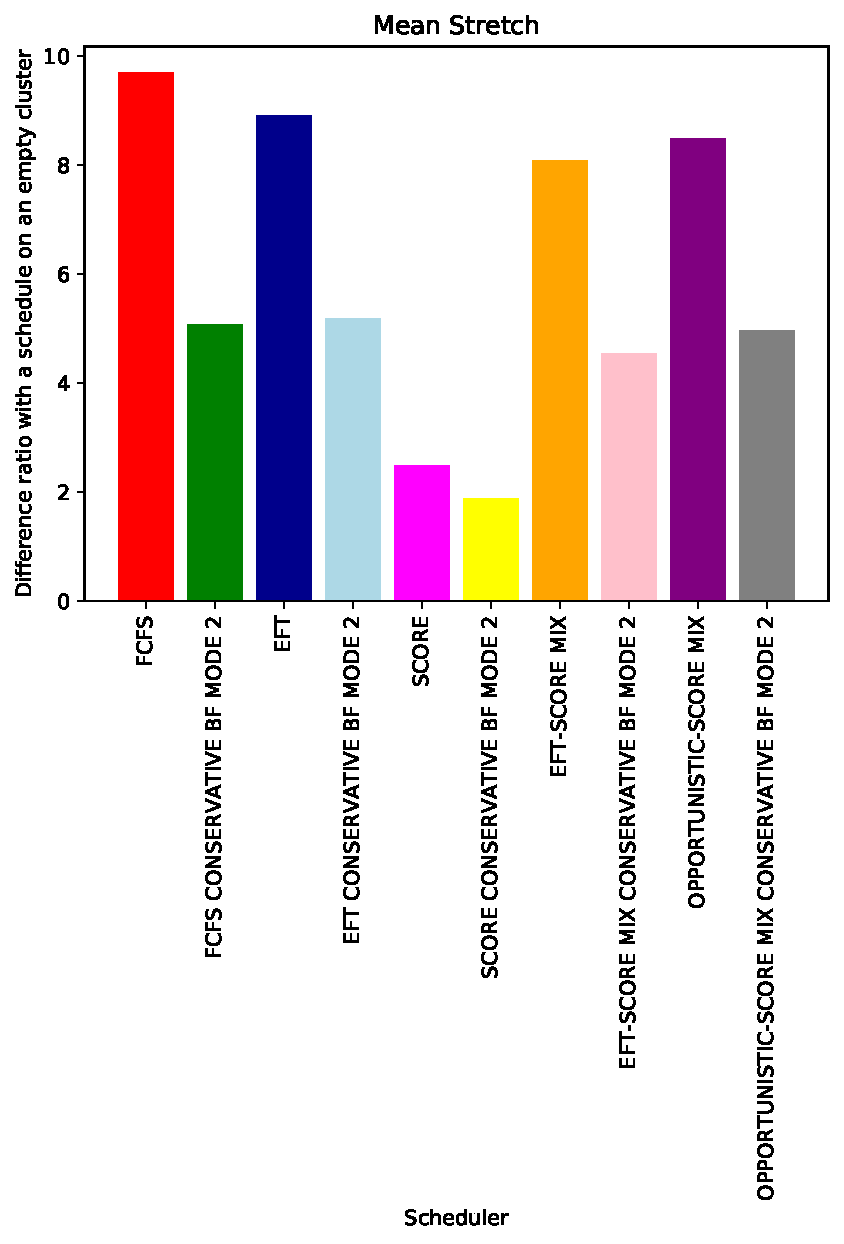
\includegraphics[width=0.9\linewidth]{MBSS/plot/Results_FCFS_Score_Backfill_2022-07-18->2022-07-18_V9271_Mean_Stretch_450_128_32_256_4_1024.pdf}\caption{Mean stretch on all jobs}\end{subfigure}
\caption{Workload of July 18}\end{figure}

\begin{figure}[H]\centering
\begin{subfigure}[b]{0.4\linewidth}\centering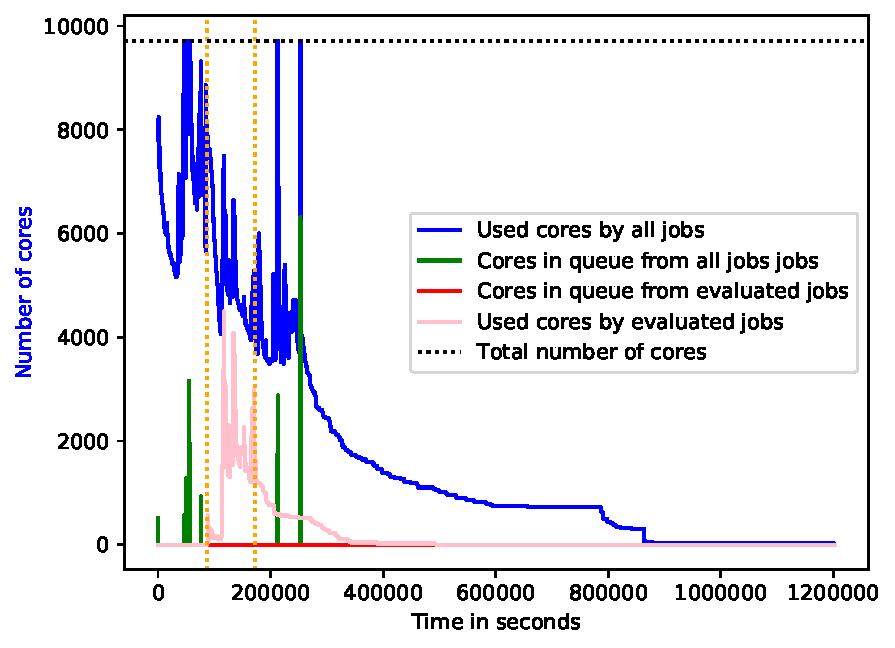
\includegraphics[width=1\linewidth]{MBSS/plot/2022-07-16->2022-07-16_V9271_Fcfs_Used_nodes_450_128_32_256_4_1024.pdf}\caption{Cluster's usage}\end{subfigure}
\begin{subfigure}[b]{0.4\linewidth}\centering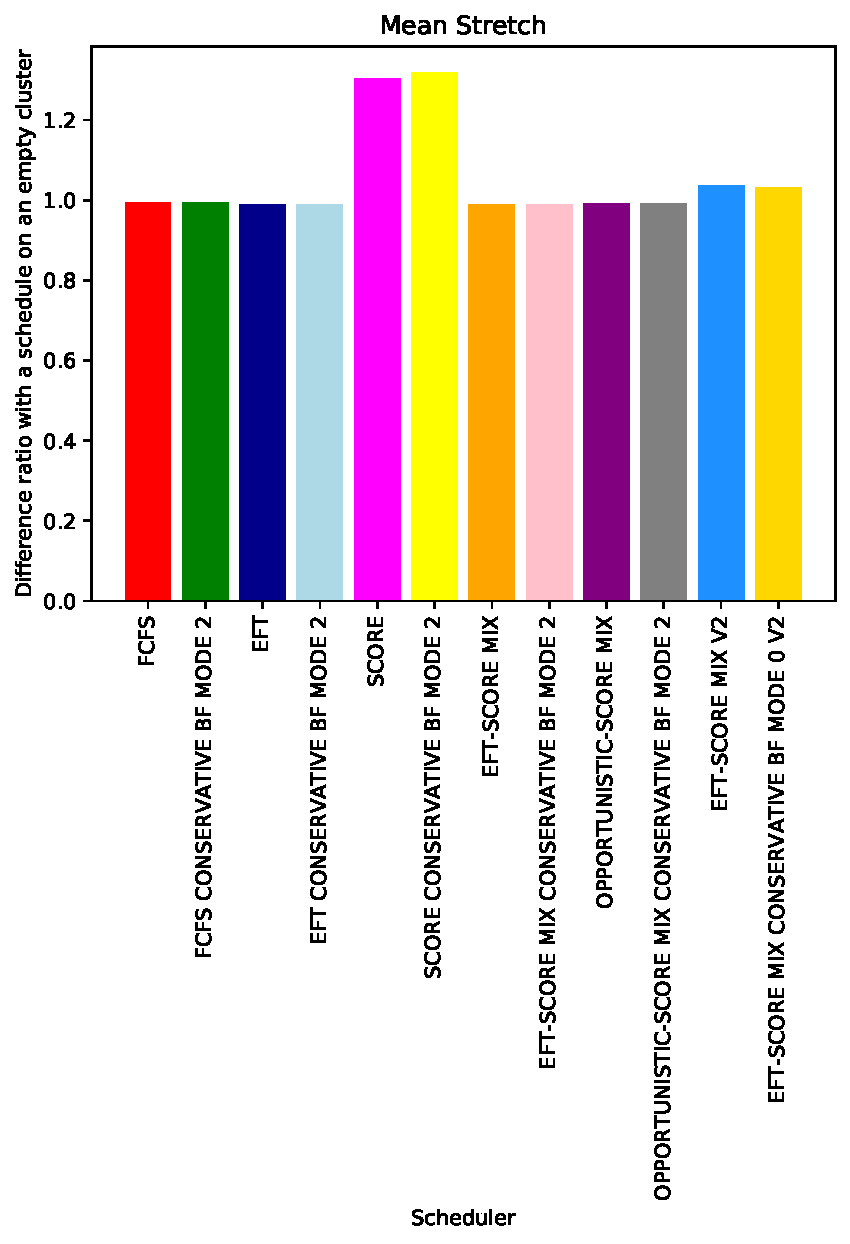
\includegraphics[width=0.9\linewidth]{MBSS/plot/Results_FCFS_Score_Backfill_2022-07-16->2022-07-16_V9271_Mean_Stretch_450_128_32_256_4_1024.pdf}\caption{Mean stretch on all jobs}\end{subfigure}
\caption{Workload of July 16}\end{figure}

\begin{figure}[H]\centering
\begin{subfigure}[b]{0.4\linewidth}\centering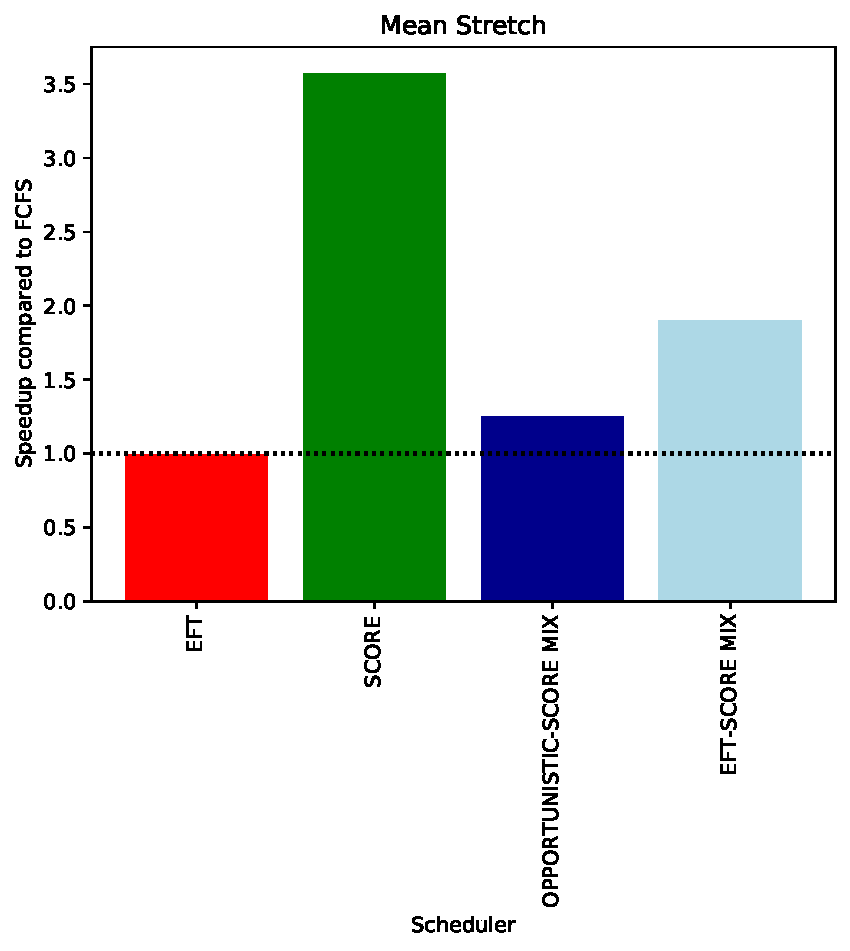
\includegraphics[width=1\linewidth]{MBSS/plot/Results_Percentage_FCFS_All_workloads_mean_Mean_Stretch_450_128_32_256_4_1024.pdf}\caption{Mean all workloads}\end{subfigure}
\begin{subfigure}[b]{0.4\linewidth}\centering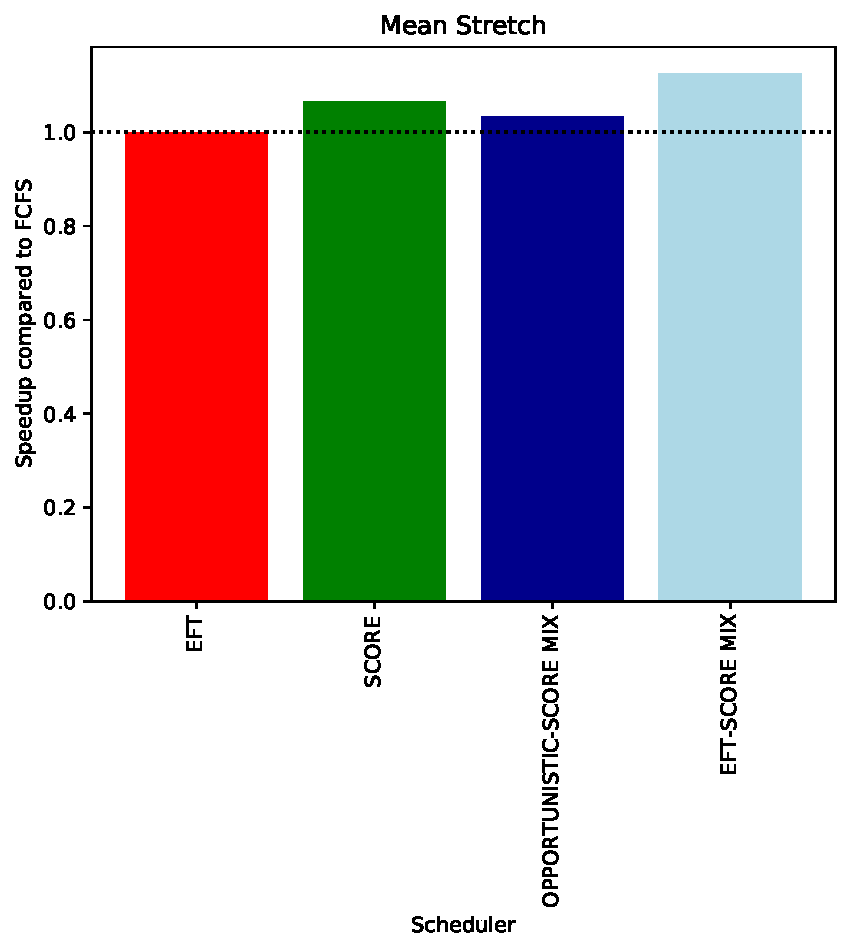
\includegraphics[width=1\linewidth]{MBSS/plot/Results_Percentage_FCFS_All_workloads_mediane_Mean_Stretch_450_128_32_256_4_1024.pdf}\caption{Median all workloads}\end{subfigure}
\begin{subfigure}[b]{0.4\linewidth}\centering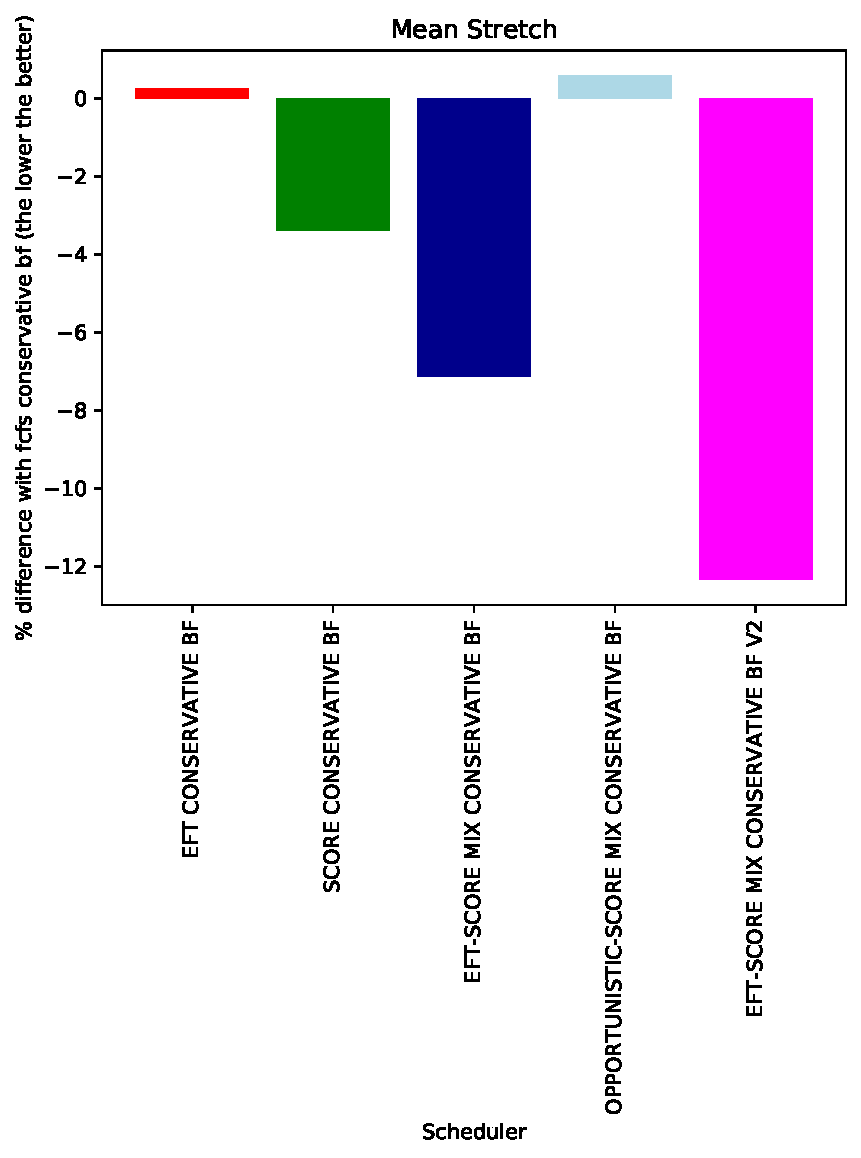
\includegraphics[width=1\linewidth]{MBSS/plot/Results_Percentage_FCFS_BF_All_workloads_mean_Mean_Stretch_450_128_32_256_4_1024.pdf}\caption{Mean all workloads with backfilling}\end{subfigure}
\begin{subfigure}[b]{0.4\linewidth}\centering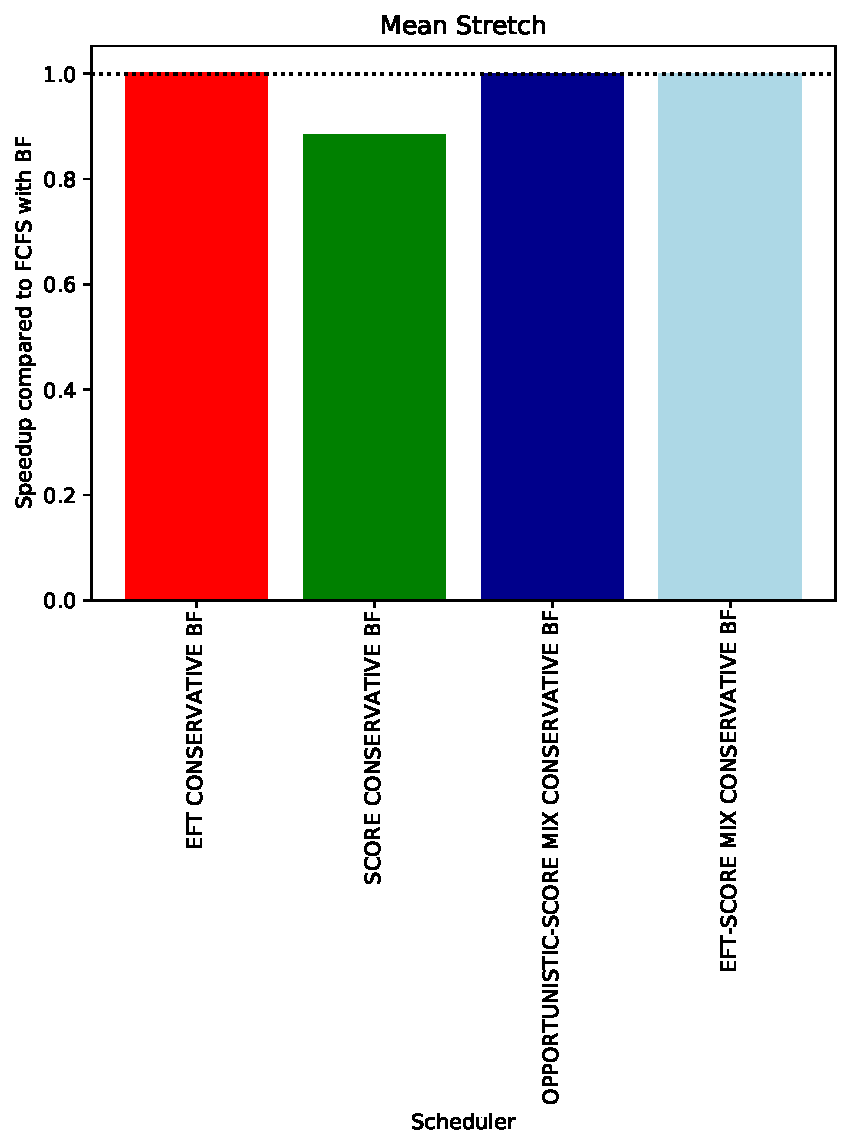
\includegraphics[width=1\linewidth]{MBSS/plot/Results_Percentage_FCFS_BF_All_workloads_mediane_Mean_Stretch_450_128_32_256_4_1024.pdf}\caption{Median all workloads with backfilling}\end{subfigure}
\caption{All workloads, mean stretch}\end{figure}

\begin{figure}[H]\centering
\begin{subfigure}[b]{0.4\linewidth}\centering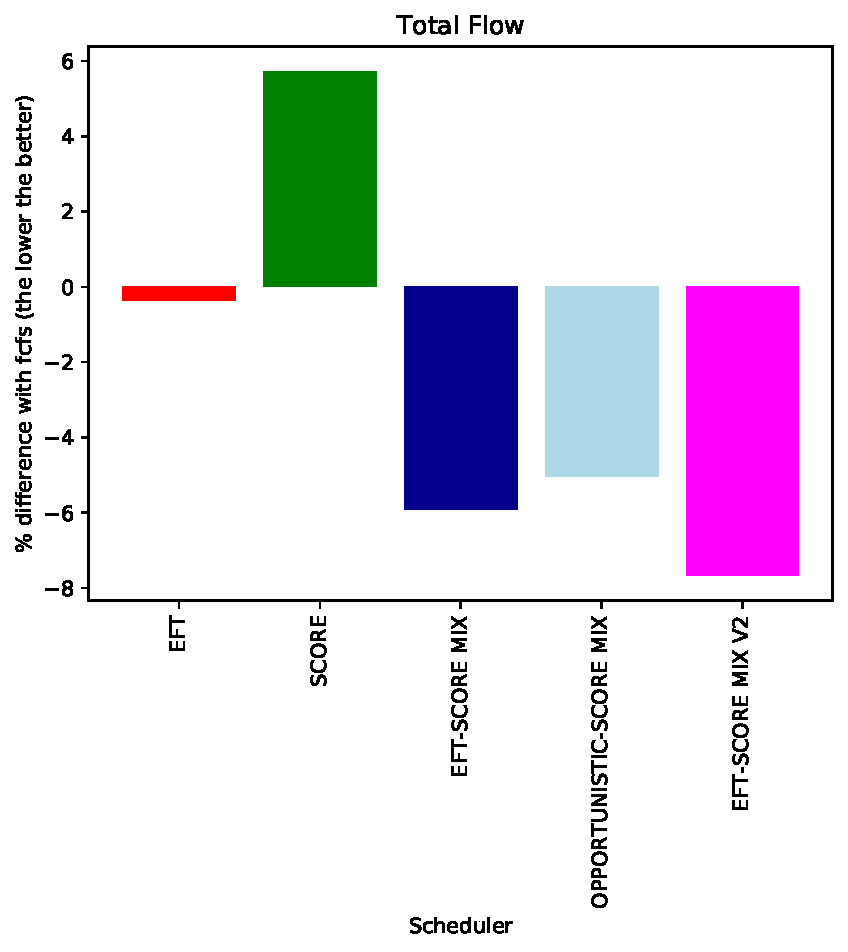
\includegraphics[width=1\linewidth]{MBSS/plot/Results_Percentage_FCFS_All_workloads_mean_Total_flow_450_128_32_256_4_1024.pdf}\caption{Mean all workloads}\end{subfigure}
\begin{subfigure}[b]{0.4\linewidth}\centering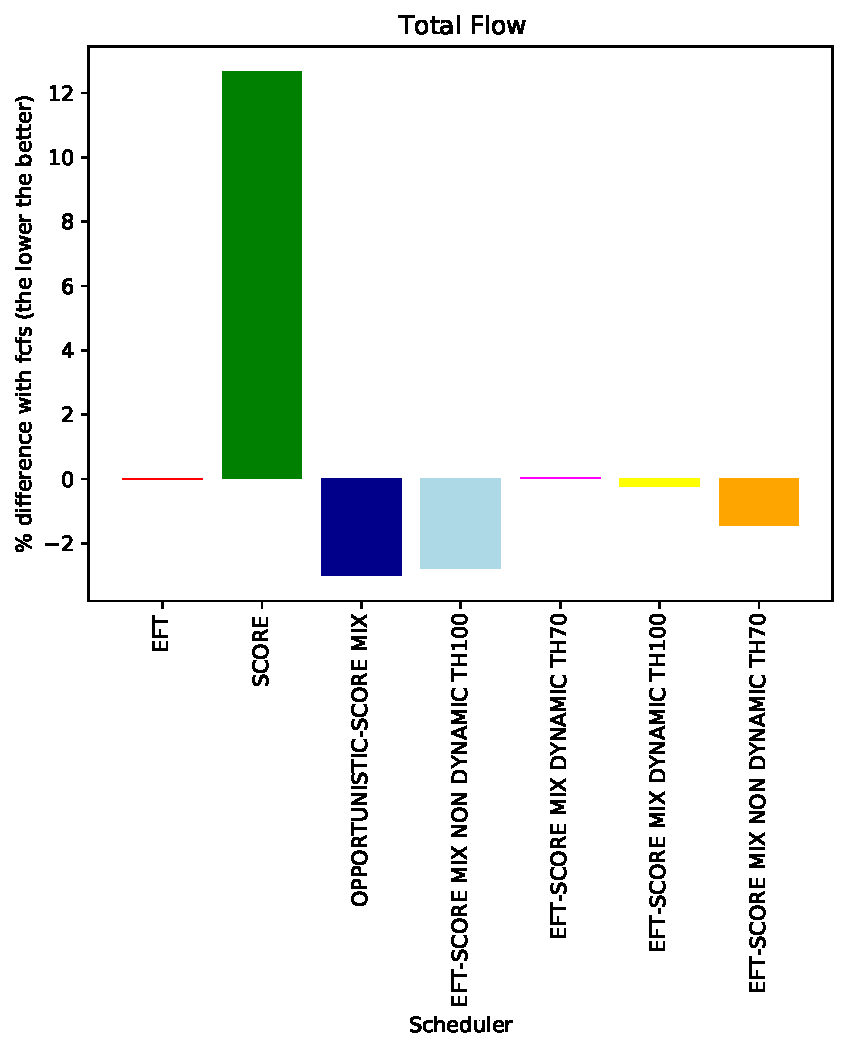
\includegraphics[width=1\linewidth]{MBSS/plot/Results_Percentage_FCFS_All_workloads_mediane_Total_flow_450_128_32_256_4_1024.pdf}\caption{Median all workloads}\end{subfigure}
\begin{subfigure}[b]{0.4\linewidth}\centering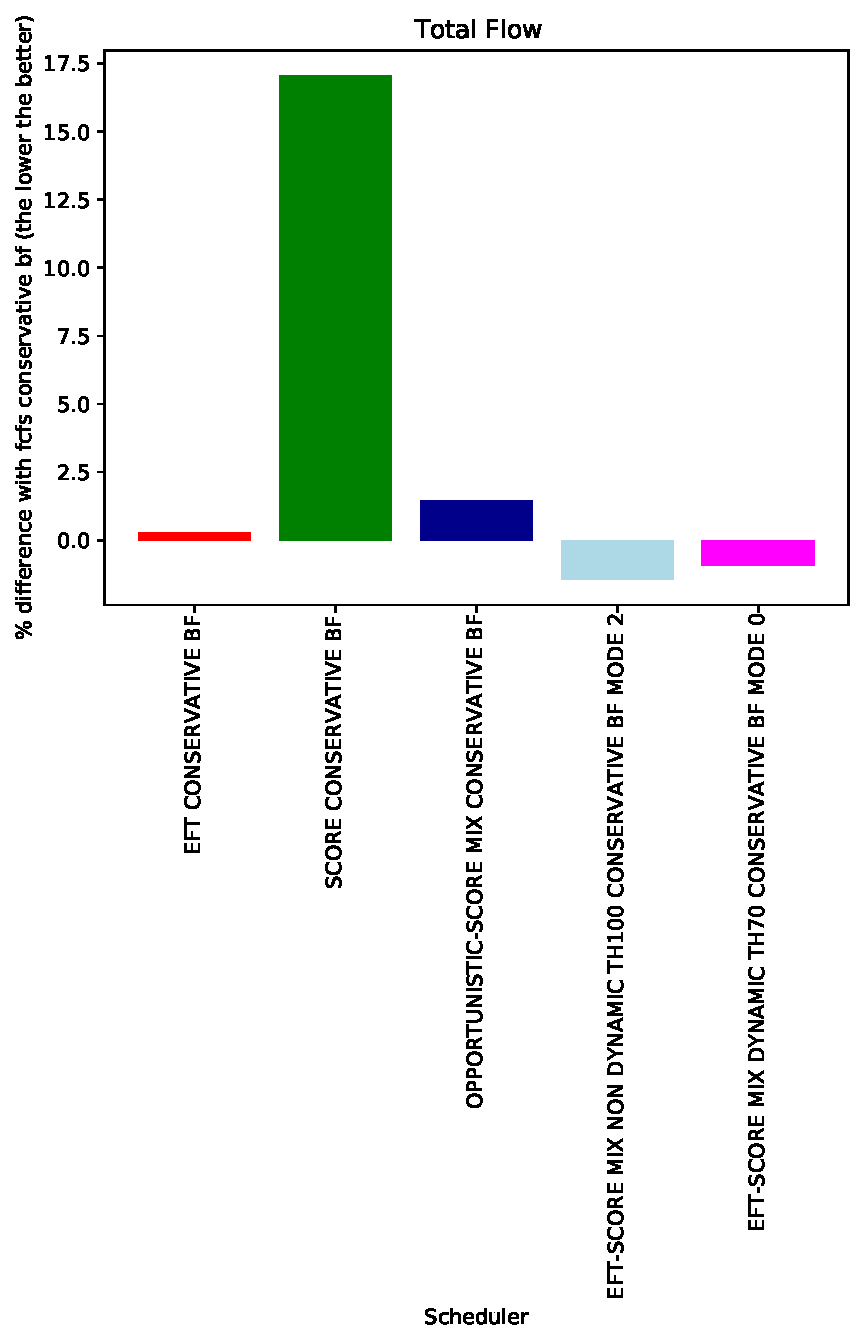
\includegraphics[width=1\linewidth]{MBSS/plot/Results_Percentage_FCFS_BF_All_workloads_mean_Total_flow_450_128_32_256_4_1024.pdf}\caption{Mean all workloads with backfilling}\end{subfigure}
\begin{subfigure}[b]{0.4\linewidth}\centering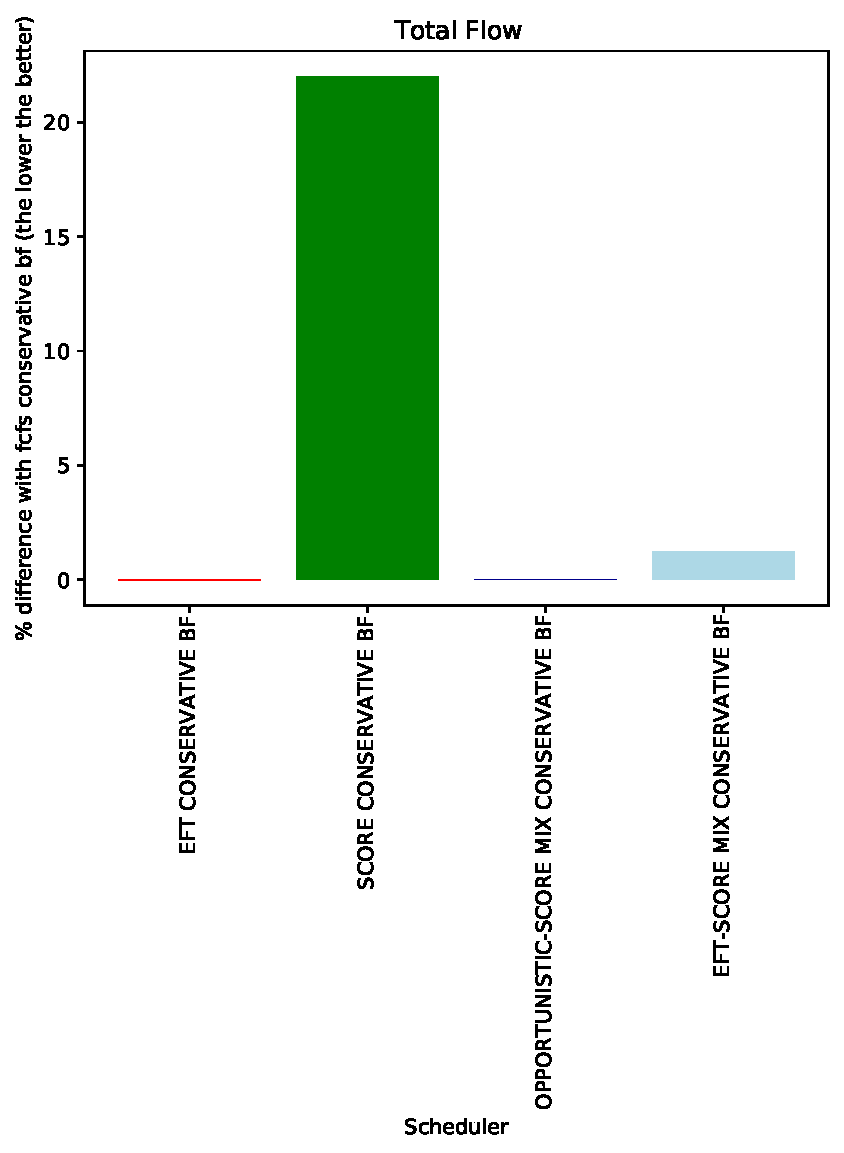
\includegraphics[width=1\linewidth]{MBSS/plot/Results_Percentage_FCFS_BF_All_workloads_mediane_Total_flow_450_128_32_256_4_1024.pdf}\caption{Median all workloads with backfilling}\end{subfigure}
\caption{All workloads, total flow}\end{figure}

\begin{figure}[H]\centering
\begin{subfigure}[b]{0.4\linewidth}\centering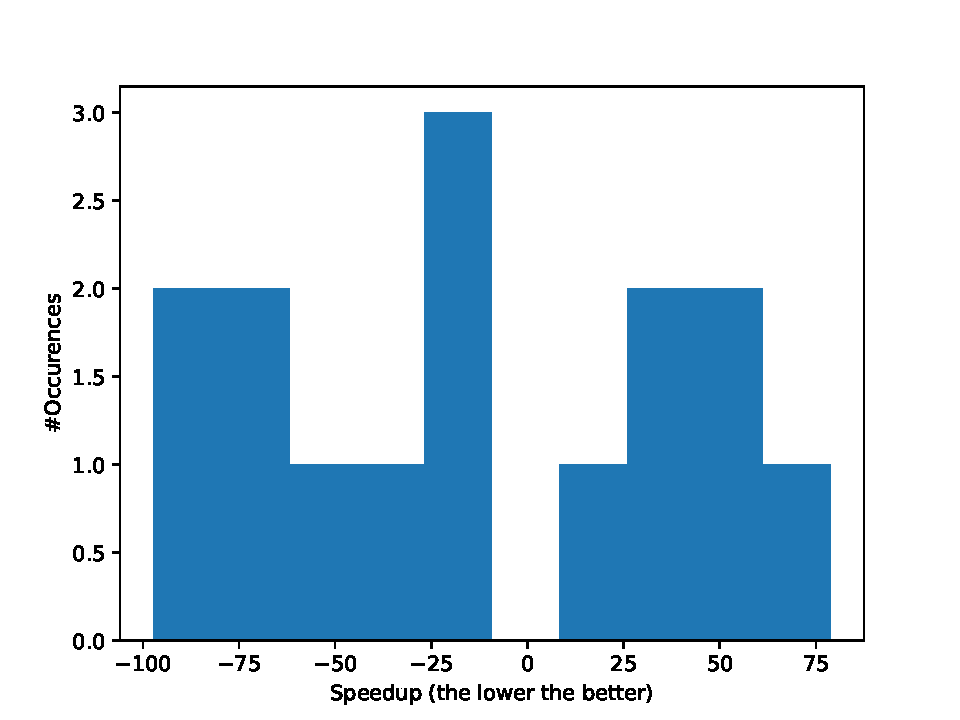
\includegraphics[width=1\linewidth]{MBSS/plot/Distribution/Stretch/Stretch_all_workloads_SCORE.pdf}\caption{SCORE}\end{subfigure}
\begin{subfigure}[b]{0.4\linewidth}\centering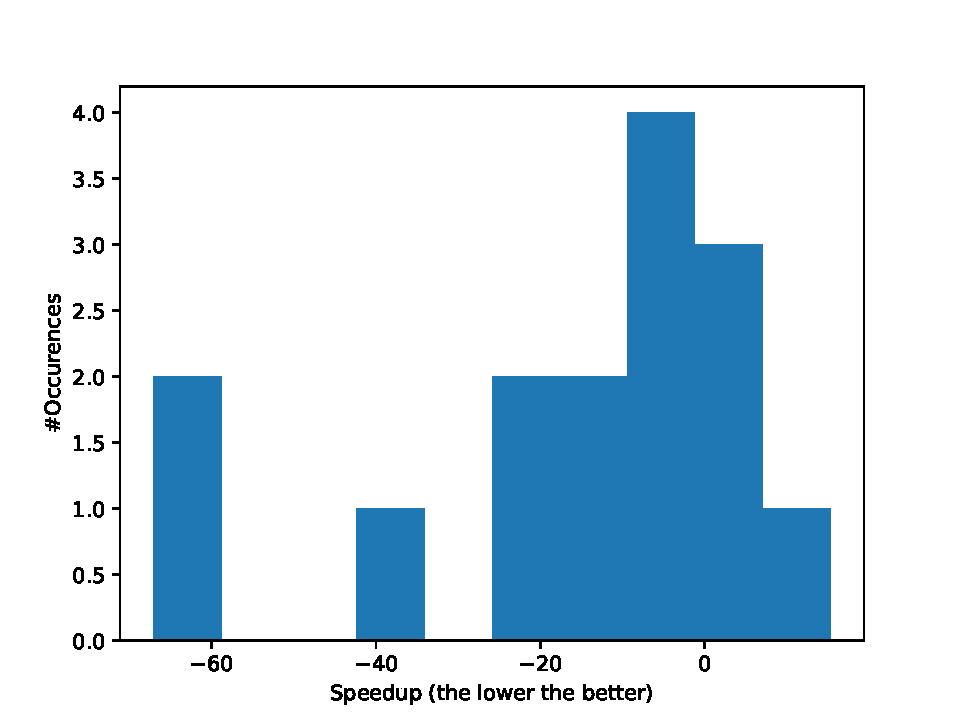
\includegraphics[width=1\linewidth]{MBSS/plot/Distribution/Stretch/Stretch_all_workloads_EFT-SCORE-MIX-NON-DYNAMIC-TH100.pdf}\caption{EFT-SCORE-MIX-NON-DYNAMIC-TH100}\end{subfigure}
\begin{subfigure}[b]{0.4\linewidth}\centering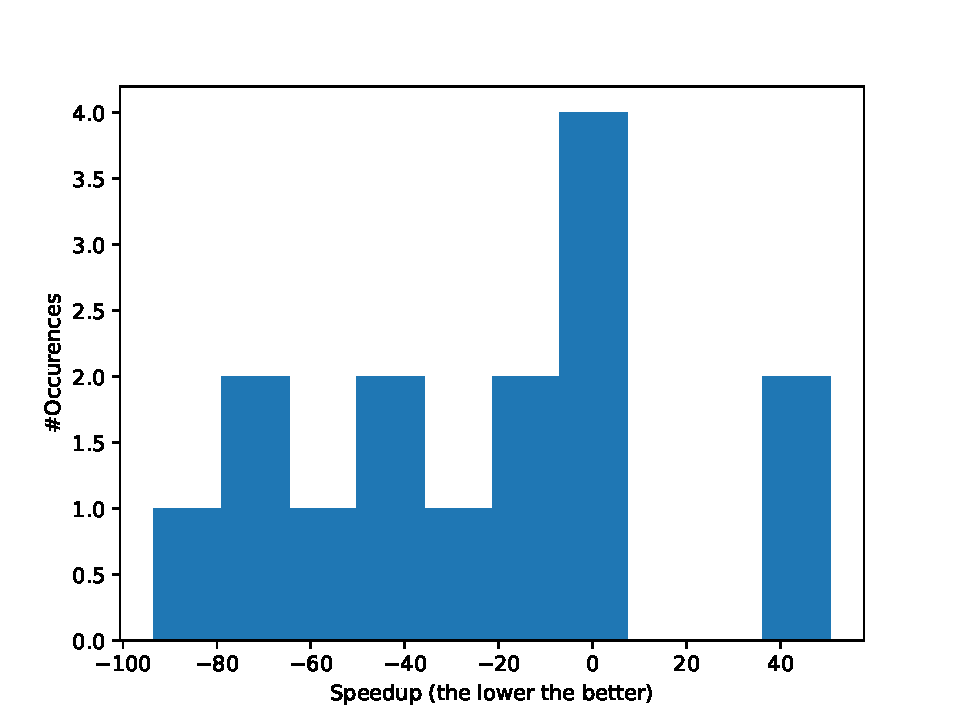
\includegraphics[width=1\linewidth]{MBSS/plot/Distribution/Stretch/Stretch_all_workloads_EFT-SCORE-MIX-DYNAMIC-TH70.pdf}\caption{EFT-SCORE-MIX-DYNAMIC-TH70}\end{subfigure}
\caption{All workloads, stretch speedup distribution}\end{figure}

\begin{figure}[H]\centering
\begin{subfigure}[b]{0.4\linewidth}\centering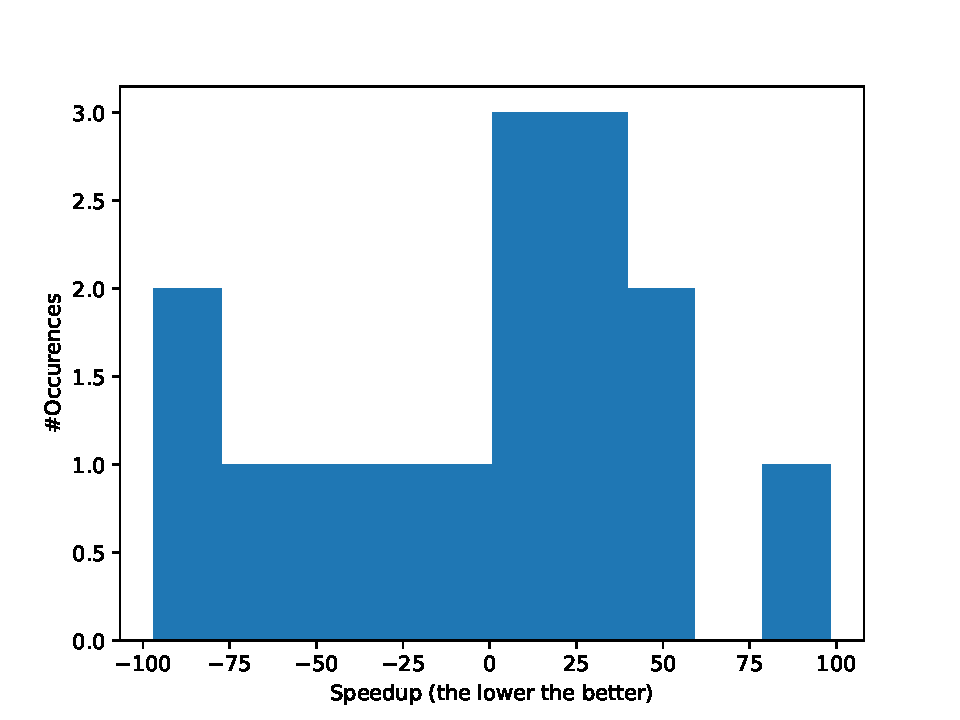
\includegraphics[width=1\linewidth]{MBSS/plot/Distribution/Stretch/Stretch_all_workloads_bf_SCORE-BF.pdf}\caption{SCORE with bf}\end{subfigure}
\begin{subfigure}[b]{0.4\linewidth}\centering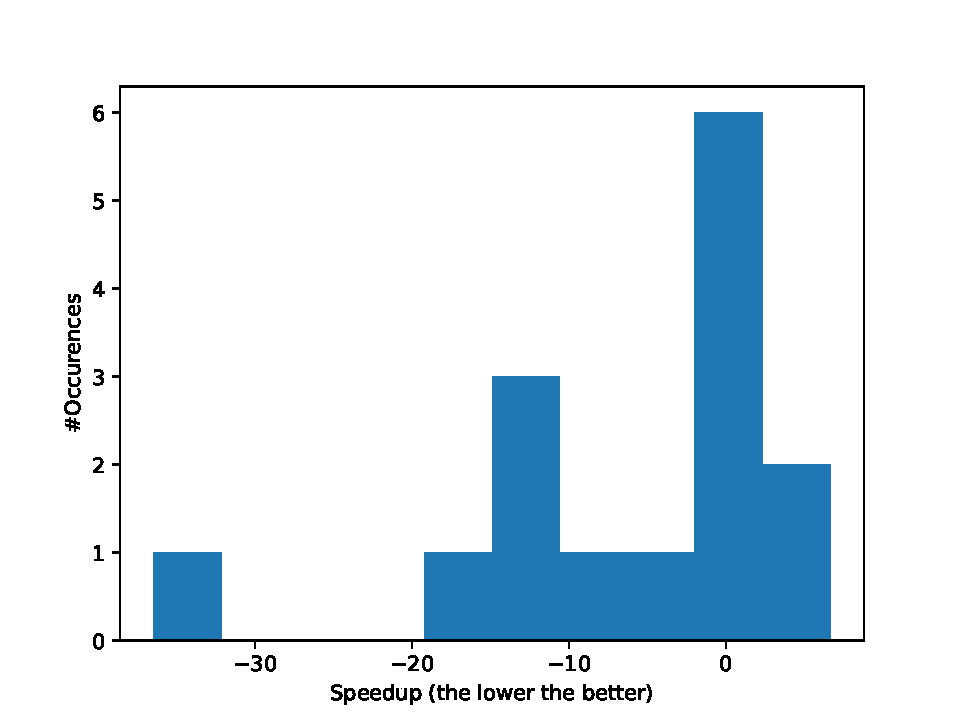
\includegraphics[width=1\linewidth]{MBSS/plot/Distribution/Stretch/Stretch_all_workloads_bf_EFT-SCORE-MIX-NON-DYNAMIC-TH100-BF.pdf}\caption{EFT-SCORE-MIX-NON-DYNAMIC-TH100-with-bf}\end{subfigure}
\begin{subfigure}[b]{0.4\linewidth}\centering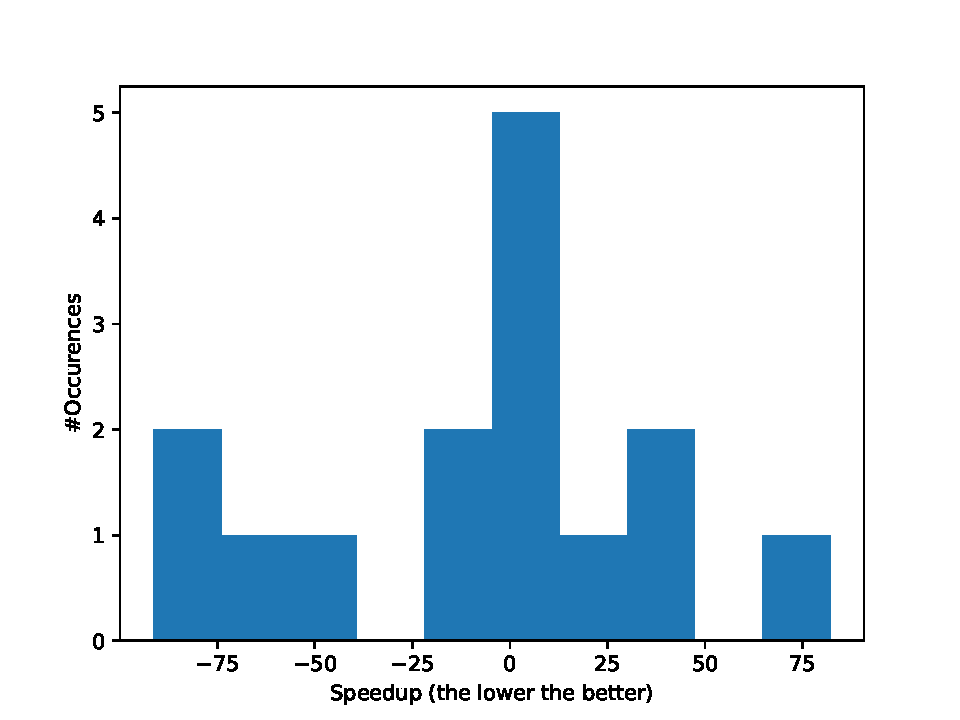
\includegraphics[width=1\linewidth]{MBSS/plot/Distribution/Stretch/Stretch_all_workloads_bf_EFT-SCORE-MIX-DYNAMIC-TH70-BF.pdf}\caption{EFT-SCORE-MIX-DYNAMIC-TH70-with-bf}\end{subfigure}
\caption{All workloads with bf, stretch speedup distribution}\end{figure}

\end{document}
